\documentclass[aspectratio=169]{beamer}

\usepackage{amssymb,amsmath}
\usepackage{graphicx}
\usepackage{url}
\usepackage{color}
\usepackage{pagenote}[continuous,page]
\usepackage{relsize}		% For \smaller
\usepackage{url}			% For \url
\usepackage{epstopdf}	% Included EPS files automatically converted to PDF to include with pdflatex

%For MindMaps
% \usepackage{tikz}%
% \usetikzlibrary{mindmap,trees,arrows}%

%%% Color Definitions %%%%%%%%%%%%%%%%%%%%%%%%%%%%%%%%%%%%%%%%%%%%%%%%%%%%%%%%%
%\definecolor{bordercol}{RGB}{40,40,40}
%\definecolor{headercol1}{RGB}{186,215,230}
%\definecolor{headercol2}{RGB}{80,80,80}
%\definecolor{headerfontcol}{RGB}{0,0,0}
%\definecolor{boxcolor}{RGB}{186,215,230}

%%% Save space in lists. Use this after the opening of the list %%%%%%%%%%%%%%%%
%\newcommand{\compresslist}{
%	\setlength{\itemsep}{1pt}
%	\setlength{\parskip}{0pt}
%	\setlength{\parsep}{0pt}
%}

%\setbeameroption{show notes on top}

% You should run 'pdflatex' TWICE, because of TOC issues.

% Rename this file.  A common temptation for first-time slide makers
% is to name it something like ``my_talk.tex'' or
% ``john_doe_talk.tex'' or even ``discrete_math_seminar_talk.tex''.
% You really won't like any of these titles the second time you give a
% talk.  Try naming your tex file something more descriptive, like
% ``riemann_hypothesis_short_proof_talk.tex''.  Even better (in case
% you recycle 99% of a talk, but still want to change a little, and
% retain copies of each), how about
% ``riemann_hypothesis_short_proof_MIT-Colloquium.2000-01-01.tex''?

\mode<presentation>
{
  \usetheme{CambridgeUS}		% bem bacana - menu superior
  \usecolortheme{default}		% branco, azul clarinho
  \useoutertheme{default}
  \useinnertheme{circles}
  \setbeamercovered{invisible}
}

\beamertemplatenavigationsymbolsempty

%% Better looking blocks
\setbeamercolor{block title alerted}{use=structure,fg=black,bg=red!80!black}
\setbeamercolor{block body alerted}{use=structure,fg=black,bg=white!90!black}

\setbeamercolor{block title}{use=structure,fg=black,bg=blue!60!white}
\setbeamercolor{block body}{use=structure,fg=black,bg=white!90!black}

\usepackage[english]{babel}
\usepackage[latin1]{inputenc}
\usepackage{subfigure}

\usepackage{times}
\usepackage[T1]{fontenc}

%% makes the ppagenote command for figure references at the end.
\makepagenote
\renewcommand{\notenumintext}[1]{}
\newcommand{\ppagenote}[1]{\pagenote[Page \insertframenumber]{#1}}


\title[GB13624]{GB13624 - Maths for Computer Science}
\subtitle[]{Lecture 2 -- Proofs, Part 2}
\author[Claus Aranha]{Claus Aranha\\{\footnotesize caranha@cs.tsukuba.ac.jp}}
\institute[COINS]{College of Information Science}
\date[2022-10-12]{2022-10-12\\{\tiny Last updated \today}}

\begin{document}

%% TODO:
% - Part 2: Induction. Slides are kinda ok, but explanation needs to be slower.
%   The point that you need to assume P(n) correct was not clear.


\begin{frame}
  \maketitle
\end{frame}

\section{Introduction}

\begin{frame}[t]{Lecture 2 -- Outline}
  In the first lecture, we covered the basic concepts of proofs. In this lecture, we first introduce a very important proof method, {\bf Induction}.\medskip
  
  After that, we discuss the concepts of {\bf state machines} and {\bf sets}.\bigskip
  
  \begin{itemize}
    \item {\bf Section 1:} Proof by Induction -- Chapter 5
    \item {\bf Section 2:} State Machines -- Chapter 5
    \item {\bf Section 3:} Sets and Relations -- Chapter 4
  \end{itemize}\bigskip

  I highly recommend that you also study chapters 6 and 7 to learn more advanced topics related to Induction and Sets.
\end{frame}

\section{Sets and Relations}

\frame{
{Part 3: Sets and Relations}

\tableofcontents[currentsection,hideallsubsections, firstsection=2, sections={2-4}]
}

\subsection{Sets: Definitions}
\begin{frame}
  \frametitle{Mathematical Set}

  \structure{Mathematical Sets} are useful when talking about proofs.\bigskip
  
  We have already used some sets: \bigskip

  \begin{itemize}
    \item $\mathbb{N}$ -- Set of natural (non negative) numbers;
    \item $\mathbb{Z}$ -- Set of integer numbers;
    \item $\mathbb{R}$ -- Set of real numbers;
  \end{itemize}
\end{frame}

\begin{frame}
  \frametitle{Characteristics of Mathematical Sets}

  \begin{itemize}
    \item  \structure{Sets} can mix different "types" of objects:
    \begin{itemize}
    \item \{7, ``Aranha'', $\pi/2$, TRUE\}
    \end{itemize}\medskip

    \item \structure{Sets} do not have a concept of "order":
    \begin{itemize}
      \item \{7, ``Aranha'', $\pi/2$, TRUE\} is the same as \item \{TRUE, 7, $\pi/2$, ``Aranha''\}
    \end{itemize}\medskip

    \item \structure{Sets} do not contain duplicates:
    \begin{itemize}
    \item \{7, $\pi$\} = \{7, $\pi$, 7\}
    \end{itemize}\medskip

    \item \structure{Sets} can be Infinite: $\mathbb{N}, \mathbb{R}, \ldots$\medskip
    
    \item The empty set: $\varnothing = \{\}$
  \end{itemize}
\end{frame}


\begin{frame}[t]{Set Membership}

  The fundamental property of a set is \structure{membership}, represented by the symbol $\in$.\bigskip

  \begin{columns}
    \column{.5\textwidth}
  Set A = \{7, TRUE, $\pi$\}
  \begin{itemize}
  \item $7 \in A$
  \item 7 is an element of $A$,
  \item 7 is in $A$,
  \item $3 \notin A$
  \end{itemize}\bigskip

  \column{.5\textwidth}
  Set B = \{7, $\mathbb{Z}$, 3\}
  \begin{itemize}
    \item $7 \in B$
    \item $7 \in \mathbb{Z}$
    \item $\mathbb{Z} \in B$
    \item \alert{$1 \notin B$}
  \end{itemize}
\end{columns}\bigskip

Note that membership is \alert{not} recursive!\bigskip

$1$ belongs to the set $\mathbb{Z}$, but $1$ does not belong to the set $B$.
\end{frame}

\begin{frame}[t]{Set Builder Notation}
  We can use \structure{Predicates} to construct sets. The set is composed of all value for which the predicate is true. For example:\bigskip 

  \begin{itemize}
  \item $A ::= \{n \in \mathbb{N} | n \text{ is a prime and } n = 4k + 1 \text{ for } k \in \mathbb{Z} \}$
  \item $B ::= \{x \in \mathbb{R} | x^3 - 3x + 1 > 0\}$
  \item $C ::= \{a^2 | a = b^2, a, b \in \mathbb{N}\}$ 
  \end{itemize}\bigskip

  Please list a few elements of each set. This looks like python's comprehension lists!
\end{frame}

\begin{frame}[t]{Set: Subsets}

  {\larger
  \begin{block}{Subset}
    \begin{itemize}
    \item $A \subset B$ means that every element of A is also an element of B
    \item $A\subset B \equiv \forall x, x\in A \rightarrow x\in B$
    \item $\mathbb{Z} \subset \mathbb{R}, \mathbb{R} \subset \mathbb{C}, \{3\} \subset \{5,3,7\}$
    \end{itemize}
  \end{block}

  \begin{block}{Important!}
    \begin{itemize}
    \item $A \subset A$
    \item Every set contains the empty subset: $\forall X, \varnothing \subset X$
    \end{itemize}
  \end{block}
  }
\end{frame}

\begin{frame}
  \frametitle{Difference between Membership and Subset}

  \begin{columns}[T]
    \column{0.5\textwidth}
    \structure{Membership} ($\in, \notin$) indicates if one member is part of a set. \structure{Subset} ($\subset, \not\subset$) indicates if one set contains the members of other sets.

    \column{0.5\textwidth}
  {\larger
  \begin{itemize}
  \item $3 \in \{3,5,6\}$
  \item $3 \not\subset \{3,5,6\}$
  \end{itemize}
  \bigskip

  \begin{itemize}
  \item $\{3\} \subset \{3,5,6\}$
  \item $\{3\} \notin \{3,5,6\}$
  \end{itemize}
  \bigskip

  \begin{itemize}
    \item \alert{$\{3\} \in \{5, 6, \{3\}\}$}
  \end{itemize}
  }
  \end{columns}
\end{frame}

\begin{frame}[t]{Power Set}
  The \structure{Power Set} of A is a special set composed of ALL subsets of A.

  \begin{equation*}
    POW(A) = \forall x \subset A, x \in POW(A)
  \end{equation*}

  For example: $POW(\{T,F\}) = \{\{T\},\{F\},\{T,F\},\varnothing\}$\vfill
    
  \alert{Check the following}: If a set $A$ is a subset of $B$, then $A$ is a member of POW$(B)$

  \begin{equation*}
    \mathbb{N} \subset \mathbb{R}, \mathbb{N} \notin \mathbb{R}, \mathbb{N} \in POW(\mathbb{R})
  \end{equation*}
\end{frame}


\begin{frame}{Operations on Sets}

  Finally, You should be familiar with the regular operations on sets:
  \bigskip

    \begin{itemize}
    \item Union: $A \cup B \rightarrow x \in A \lor x \in B$\bigskip
    \item Intersection: $A \cap B \rightarrow x \in A \land x \in B$\bigskip
    \item Subtraction: $A - B \rightarrow x \in A \land x \notin B$\bigskip
    \item Complement: $\overline{A} = D - A$, where $D$ is the \structure{domain}\\ (the "everything" set or "parent" set of interest).
    \end{itemize}
\end{frame}

\subsection{Sets and Proofs}

\begin{frame}[t]{Example of proofs using sets (1)}

  \begin{proof}[Prove that the empty set is a subset of every set.]
    Proof by construction:

  \begin{enumerate}

  \item $A \subset B$ means that $\forall x, x \in A \rightarrow x \in B$\bigskip

  \item If $A = \varnothing$ then $x \in A$ is FALSE for $\forall x$, so we can replace ``$\forall x \in A$'' with FALSE in {\bf (1)}\bigskip

\item The statement FALSE $\rightarrow x \in B$ is always TRUE.\\ \hfill (remember that FALSE $\rightarrow X$ is always TRUE)\bigskip

  \item Therefore, $\varnothing \subset B$ is TRUE $\forall B$
  \end{enumerate}
  \end{proof}
\end{frame}


\begin{frame}[t]{Sets and Proofs Example (2)}

  \begin{equation*}
    A \cup (B \cap C) \iff (A \cup B) \cap (A \cup C)
  \end{equation*}

  \begin{proof}[Proof that Union and Intersection are Distributive]
    Proof by sequence of "IFF"s:
    \begin{enumerate}
    \item \structure{$x \in A \cup (B \cap C)$} {\bf iff}
    \item $x \in A \lor x \in (B \cap C)$ {\bf iff} \hfill (definition of union)
    \item $x \in A \lor (x \in B \land x \in C)$ {\bf iff} \hfill
      (definition of intersection)
    \item $(x \in A \lor x \in B) \land (x\in A \lor x \in C)$ {\bf
      iff} \hfill (distributive prop.)
    \item $(x \in A\cup B) \land (x \in A\cup C)$ {\bf iff}\hfill
      (definition of union)
    \item \structure{$x \in (A\cup B)\cap (A\cup C)$}  \hfill
      (defintion of intersection)

    \end{enumerate}
  \end{proof}
\end{frame}

\begin{frame}[t]{Sequences and Sets}
  A \alert{sequence} is another kind of mathematical object. It is similar to a set, but \alert{different in important ways.}\bigskip 

  \begin{itemize}
  \item Sequences are represented by parenthesis: $(1, 2, 1), (T, F)$
  \item Sequences can have repeated elements: $(T, T, T, F, F)$
  \item The order of elements in a sequence is important: $(0, 1) \neq (1, 0)$
  \end{itemize}\bigskip 

  We often see sequences as the products of \structure{multiplication between sets}:\bigskip

  \begin{itemize}
    \item All binary sequences with 3 elements: $\{0,1\}^3 = (0, 0, 0), (0, 0, 1), \ldots (1, 1, 1)$
    \item All pairs of two natural numbers: $\mathbb{N}^2 = (0, 0), (0, 1), (0, 2), (0, 3) \ldots (100, 7) \ldots$
  \end{itemize}
\end{frame}


\subsection{Binary Relations}
\begin{frame}
  \frametitle{Definition of Binary Relations}
  \structure{Binary Relations} define an association of elements from one set (the {\bf domain}) to another set (the {\bf co-domain}). We see (binary) relations in many different situations:\bigskip

  \begin{itemize}
    \item Functions are a special case of binary relations: f(x) = y.
    \begin{itemize}
      \item A function associates the set of inputs with the sets of outputs;
    \end{itemize}\bigskip

    \item Operations such as set membership can be expressed as binary relations.
    \begin{itemize}
      \item For example, the predicate \structure{$P(x): x \text{ is prime}$} defines a binary relation from $\mathbb{N}$ to \{TRUE, FALSE\}
    \end{itemize}\bigskip

    \item "Relational Databases" (for example, SQL) are also based on the idea of binary relations
    \begin{itemize}
      \item Key of X, member of a table, joint key, etc;
    \end{itemize}
    \end{itemize}
\end{frame}

\subsection{Binary Relation Definitons}

\begin{frame}[t]{Example of Binary Relation}
  Relation \structure{$P(x): x \text{ is prime}$}:\bigskip

  \begin{itemize}
  \item Domain: $x \in \mathbb{N}$
  \item Co-Domain: $P(x) \in \{True, False\}$ 
  \item Examples:\\ $P(1) = False$\\ $P(3) = True$\\$P(13) = True$\\$P(20) = False$
  \end{itemize}\bigskip 

  It is common to represent binary relations as a graph between the \structure{domain} and the \structure{co-domain}.


\end{frame}

\begin{frame}[t]{Binary Relations as a Graph}

  \begin{columns}[t]
    \column{0.4\textwidth}
    Let's consider the binary relation {\bf R} from a set of students {\bf (D)} that are registered to a set of courses {\bf (J)}.\bigskip

    \begin{itemize}
    \item \structure{Domain}: Set of students;
    \item \structure{Co-domain}: Set of courses;
    \item \alert{Vertices:} Domain and Co-domain are represented as vertices;
    \item \alert{Edges:} Directed edges from Domain to Co-domain;
    \end{itemize}\bigskip

    \column{0.6\textwidth}

    \begin{center}
      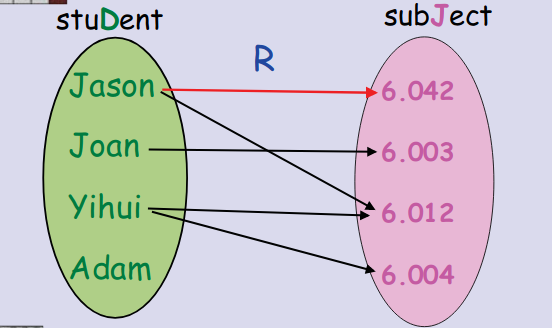
\includegraphics[width=0.6\textwidth]{../img/relations}
    \end{center}\pagenote{Relation Graph Image from MIT OCS}
    Notation to describe the relation:
    \begin{itemize}
    \item $R($Jason$) = \{6.042, 6.012\}$
    \item Jason $R$ 6.042
    \item $R(\{$Jason, Yihui$\}) = \{6.042, 6.012, 6.004\}$
    \end{itemize}
  \end{columns}
\end{frame}


\begin{frame}{Relations and Inverse Relations}

  If we think of a binary relation as a directed graph, the \structure{Inverse Relation} is the relation defined by the same graph when the edges are reversed:\bigskip

  Relation $R$:
  \begin{equation*}
    R(X) ::= {j \in J | \exists d \in X, d R j}
  \end{equation*}

  Reverse Relation $R^{-1}$:
  \begin{equation*}
    R^{-1}(Y) ::= {d \in S | \exists j \in Y, d R j}
  \end{equation*}
  \bigskip

  \begin{columns}
    \column{0.5\textwidth}
    \begin{itemize}
      \item $R(Jason) = \{6.042, 6.012\}$
      \item $R^{-1}(6.012) = \{Jason, Yihui\}$
    \end{itemize}
    \column{0.5\textwidth}
    \begin{center}
      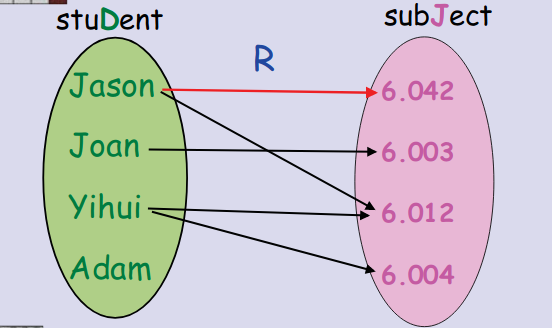
\includegraphics[width=0.6\textwidth]{../img/relations}
    \end{center}
  \end{columns}
\end{frame}

\begin{frame}[t]{Composite Relations}

  \begin{columns}[t]

    \column{0.5\textwidth}
    If we have a relation $V$ from set $P$ to set $D$, and a relation $R$ from set $D$ to set $J$, then we can define a \structure{composite} relation $R\circ V$ from set $P$ to set $J$ (we can also use $R(V)$).\bigskip

    \begin{itemize}
    \item $R(V(X))$ or $(R\circ V)(X)$
    \item $R(V(\text{FTL})) = \{6.003\}$
    \begin{itemize}
      \item professor FTL super{\bf V}ises Joan;\bigskip

      \item Joan is {\bf R}egistered to class 6.003;\bigskip

      \item professor FTL {\bf VR} 6.003 (superregister?)
    \end{itemize}
    \end{itemize}


    \column{0.5\textwidth}
    \begin{center}
      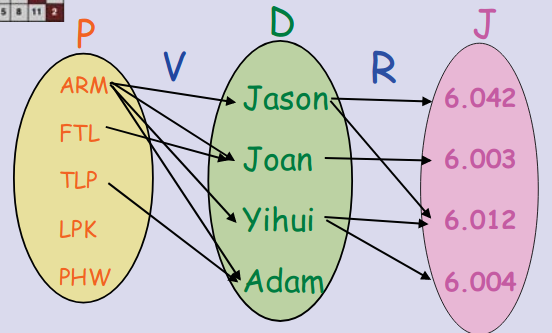
\includegraphics[width=0.8\textwidth]{../img/composite_relation}
    \end{center}

  \end{columns}
\end{frame}


\begin{frame}{Types of Binary Relations}

  We can classify a binary relation based on the number of degrees (arrows) in the relation graph. Imagine a relation $R$ from $X$ to $Y$ (i.e.: $R(X) = Y$)\bigskip

  Classification of $R$ based on $Y$:
  \begin{itemize}
  \item {\bf Surjection}: Every element in $Y$ has $\geq 1$ in-arrows. (Every Y has {\bf one or more} X)
  \item {\bf Injection}: Every element in $Y$ has $\leq 1$ in-arrows. (Every Y has {\bf one or less} X)
  \end{itemize}\smallskip

  Classification of $R$ based on $X$:
  \begin{itemize}
  \item {\bf Total}: Every element in $X$ has $\geq 1$ out arrows. (Every $X$ has {\bf one or more} $Y$)
  \item {\bf Function}: Every element in $X$ has $\leq 1$ out arrows. (Every $X$ has {\bf one or less $Y$})
  \end{itemize}\smallskip

  An important definition:
  \begin{itemize}
  \item {\bf Bijection}: Every element of $X$ has {\bf exactly one} element of $Y$, {\bf and vice versa}.
  \end{itemize}
\end{frame}

\begin{frame}
  \frametitle{Types of Binary Relations: Examples}

    \begin{block}{Example 1: $g: \mathbb{R}\times\mathbb{R} \rightarrow \mathbb{R}, g(x,y) = 1/(x-y)$}
      \begin{itemize}
      \item This is a {\bf function}, because each pair $(x,y)$ has at most one output.
      \item This is not {\bf total}, because not every pair $(x,y)$ has an output: $(x = y)$ has no output.
      \end{itemize}
    \end{block}

    \begin{block}{Example 2: $g_o: \mathbb{R}\times\mathbb{R} - \{x,y|x=y\} \rightarrow \mathbb{R}, g_o(x,y) = 1/(x-y)$}
      \begin{itemize}
      \item $g$ and $g_o$ are similar relations, but defined on different domains.
      \item The domain of $g_o$ removes all $(x,y)$ where $x = y$
      \item Because of this, $g_0$ is {\bf function} (every pair has at most one output) and {\bf total} (every pair has at least one output).
      \end{itemize}

    \end{block}

\end{frame}

% \begin{frame}
%   \frametitle{Size of Finite Sets}
%
%   {\larger
%     We can use the characteristics of relations to estimate the
%     size of sets (domains and co-domains).
%
%     \vfill
%
%     \begin{itemize}
%     \item A bijection B $\rightarrow |A| = |B|$
%     \item A function surjection B $\rightarrow |A| \geq |B|$
%     \item A total injection B $\rightarrow |A| \leq |B|$
%     \end{itemize}
%   }
% \end{frame}
%
% \begin{frame}
%   \frametitle{Set Size Example: Finite power sets and binary strings}
%
%   {\larger
%     What is the size of the Power Set of a \structure{finite} set?
%
%     \vfill
%
%     \begin{itemize}
%     \item Make a bijection between the power set and the binary string
%     \item Calculate the size of a binary string
%     \item Establish equality
%     \end{itemize}
%
%   }
% \end{frame}

\section{Induction}

\frame{
{Part 1: Induction}

\tableofcontents[currentsection,hideallsubsections, firstsection=2, sections={2-4}]
}

\subsection{Introductory Examples}



\begin{frame}{An initial induction (1/2)}
  Imagine that I want to color the natural numbers ($\mathbb{N} \geq 0$), using the following rules:\bigskip

  \begin{itemize}
    \item Number $0$ is \alert{red}
    \item Any integer next to a \alert{red} number is also \alert{red}
  \end{itemize}\bigskip

  Using these rules, can you imagine how the set $\mathbb{N}$ looks like?
\end{frame}

\begin{frame}{An initial induction (2/2)}

  \begin{center}
    Result: \alert{0,1,2,3,4,...}
  \end{center}\bigskip

  The "rule of reds" gives us a general idea of induction:

  \begin{itemize}
  \item $R(0)$ is True
  \item $R(0) \rightarrow R(1); R(1) \rightarrow R(2); R(2) \rightarrow R(3); \ldots$
  \item $R(n) \rightarrow R(n+1)$ for every $n \in \mathbb{N}$
  \end{itemize}\bigskip

  Induction can be used to prove a predicate that depends on some $n \in \mathbb{N}$.
  \begin{equation*}
    \frac{R(0), R(n)\rightarrow R(n+1), n\in\mathbb{N}}{\forall n, R(n)}
  \end{equation*}
\end{frame}

\begin{frame}{Example of proof by Induction}

  Let's prove that:
  \begin{equation*}
    P(n): 1 + r + r^2 + r^3 + \ldots + r^n = \frac{r^{n+1}-1}{r-1}, r \neq 1, \forall n \in \mathbb{N}
  \end{equation*}\bigskip

  Remember the modus ponens rule for induction:
  \begin{equation*}
    \frac{P(0), P(n)\rightarrow P(n+1), n\in\mathbb{N}}{\forall n, P(n)}
  \end{equation*}\bigskip

  To prove the bottom part, we need to prove all statements in the top part are true.

  \begin{itemize}
  \item First Step: Prove $P(0)$
  \item Second Step: Prove $P(n) \rightarrow P(n+1)$
  \end{itemize}
\end{frame}

\begin{frame}{Example of proof by Induction}

  \begin{proof}[Proof of $P(n), \forall n \in \mathbb{N}$ by induction on $n$]
    {\bf First Step:} Prove $P(0)$
    \begin{itemize}
    \item $P(0)$, left side: $r^0 = 1$
    \item $P(0)$, right side: $\frac{r^{0+1}-1}{r-1} = \frac{r-1}{r-1} = 1$
    \end{itemize}\medskip

    {\bf Second Step:} Prove $P(n) \rightarrow P(n+1)$
    \begin{itemize}
    \item $P(n+1)$, left side: $1 + r + r^2 + \ldots + r^n + r^{n+1}$, which is equal to $P(n)+r^{n+1}$
    \item Because $P(n)$ is True, $P(n)+r^{n+1} = \frac{r^{n+1}-1}{r-1} + r^{n+1} = \frac{(r^{n+1}-1)}{r-1} + \frac{(r^{n+1}(r-1))}{r-1}$
    \item Algebra: $\frac{(r^{n+1}-1) + (r^{n+1}(r-1))}{r-1} = \frac{r^{n+1} - 1 + r^{n+2} - r^{n+1}}{r-1} = \frac{r^{n+2} - 1 + (r^{n+1} - r^{n+1})}{r-1}$
    \item $\frac{r^{n+2} - 1}{r-1} = \frac{r^{(n+1)+1} - 1}{r-1}$, which is the right side of $P(n+1)$
    \end{itemize}
  \end{proof}
\end{frame}

\subsection{Proof by Induction}
\begin{frame}[t]{Review: Proof Template for Induction}

  {\larger
    {\bf Proof by induction on $n$}\\
    Proof hypothesis: $P(n) = \ldots$ for all $n \in \mathbb{N}. n \geq 0$\\

    \bigskip

    First we prove $P(0)$.\\
    $\ldots$ \emph{(calculate that P(0) is True)}\\
    $\ldots$\\

    \bigskip

    Second we prove that $\forall n \geq 0, P(n) \rightarrow P(n+1)$\\
    $\ldots$ \emph{(calculate P(n+1) using P(n))}\\
    $\ldots$\\

    \bigskip

    This completes the proof that $P(n)$ for all $n\in\mathbb{N}$\hfill$\qed$
  }
\end{frame}

\subsection{The Statue Park}

\begin{frame}[t]{The Statue Park}{A more complex proof by induction}

  The university is making a new park with the following rules:
  \begin{itemize}
    \item The park is square, with side $2^n$;
    \item In the middle of the park, there is a statue, size $1\times 1$;
    \item Other than that, the park is made of L-shaped tiles, with size $3m^2$;
  \end{itemize}\bigskip

  How can we prove that it is possible to build this park for any $n$?
\end{frame}

\begin{frame}[t]{The Statue Park}{Drawing Proof}
  Remember the rule of induction:
  \begin{itemize}
    \item Prove that $P(0)$ is true.
    \item Assume that $P(n)$ is true, then prove that $P(n) \implies P(n+1)$
  \end{itemize}
\end{frame}


\subsection{BAD induction proof}

\begin{frame}[t]{BAD Proof by induction: All horses are of the same color}

  $P(n) ::=$ for any \structure{set} with \alert{exactly n horses}, all horses have the same color.\bigskip

  \begin{itemize}

  \item<2-> {\bf Prove P(1)}: For any set with one horse, all horses have the same (one) color.

  \item<3-> {\bf Assume P(n) is true:} For any set with $n$ horses, all horses have the same color.
  \item<4-> {\bf Show that $P(n) \implies P(n+1)$:}
    \begin{itemize}
    \item <5->Consider the set of n+1 horses: $H = h_1, h_2, \ldots, h_n, h_{n+1}$
    \item <6->Subset A ($h_1, h_2, \ldots, h_n$): has $n$ horses, so all horses have the same color.
    \item <7->Subset B ($h_2, \ldots, h_n, h_{n+1}$): \alert{also} has $n$ horses, so all horses have the same color.
    \item <8->Horse $h_2$ is in subset $A$ {\bf and} in subset $B$, so subset $A$ and $B$ have the same color.
    \end{itemize}
  \item<9-> Since we showed that P(n+1) is true if P(n) is true, then all horses for any group size have the same color.
  \end{itemize}\bigskip

  \only<10>{\alert{QUIZ}: What is wrong with this proof?}
\end{frame}

\begin{frame}{What is wrong with the horse proof?}

  The induction step when we show that $P(n) \implies P(n+1)$ is not valid.\bigskip

  \begin{itemize}
    \item The implication proof depends on "$h_i$ belongs to subsets $A$ and $B$".
    \item But is this ALWAYS true?
    \begin{itemize}
      \item When $n+1 = 2$, The $n+1$ set is $\{h_1, h_2\}$, set $A = h_1$, set $B = h_2$;
      \item But in this case, {\bf there is no $h_i$ that is common to $A$ and $B$}!
    \end{itemize}
    \item So the implication proof is not valid when $P(2)$.
  \end{itemize}\bigskip

  Note that this is the only problem with the proof!
\end{frame}

\subsection{Strong Induction}

\begin{frame}[t]{Strong Induction}

  {\larger
    \begin{itemize}
    \item In regular induction, you assume P(n) to show P(n+1)

      \bigskip

    \item In strong induction, you assume P(0), P(1), P(2) \ldots
      P(n), and use all of them to show P(n+1)
    \end{itemize}
  }
\end{frame}

\begin{frame}
  \frametitle{Strong Induction Example: Stacking Game}
  {\larger
  \begin{itemize}
  \item Begin with a stack of 10 blocks
  \item Divide it in two (a, b): for example, 2 and 8 blocks.
  \item For each division, you get $a\times b$ points: 16 points
  \item Repeat with the new stacks until all stacks have 1 block.
  \end{itemize}

  \bigskip

  \alert{Which of the two strategies below give you more points?}
  \begin{itemize}
  \item Simple strategy: $(1 \times 9)$ + $(1 \times 8)$ + $(1 \times 7)$ + $(1 \times 6)$... \only<2->{45 points!}
  \item CS recursive strategy: $(5 \times 5)$ + $(2 \times 3)$ + $(2 \times 3)$, ... \only<3->{45 points!}
  \end{itemize}
  }
\end{frame}

\begin{frame}
  \frametitle{Proof: All strategies have the same score (Part I)}

  {\larger
  Let us prove by strong inductions that {\bf ALL} strategies for the \alert{stack
  game with ``n'' blocks} have the same final score:
  \begin{equation*}
    C(n) = \frac{n(n-1)}{2}
  \end{equation*}

  \bigskip

  {\bf Base Cases: 0, 1}
  \begin{itemize}
  \item When the stack has 0 blocks, I have no moves, so 0 points.
  \item When the stack has 1 block, I have no moves, so 0 points.
  \end{itemize}
  \begin{equation*}
    C(0) = \frac{0(0-1)}{2}, C(1) = \frac{1(1-1)}{2} = 0
  \end{equation*}
  }
\end{frame}

\begin{frame}
  \frametitle{Proof: All strategies have the same score (Part II)}

    {\bf Inductive Case} $C(n+1)$\\
    By strong induction, we assume that all $C(0)\ldots C(n)$ are true.

    \bigskip

    \begin{enumerate}
    \item A stack with $n+1$ blocks can be split into two: $k$ and $n+1-k$\medskip

    \item The score is: $C(n+1) = (k\times(n+1-k)) + C(k) + C(n+1-k)$\medskip

    \item Using the strong inductive assumption: $\forall m \leq n, C(m) = \frac{m(m-1)}{2}$\medskip
    
    \item Transforming (2): $C(n+1) = \frac{2k(n+1-k)}{2} + \frac{k(k-1)}{2} +
      \frac{(n+1-k)(n-k)}{2}$
  \end{enumerate}\bigskip

  ... You can finish the calculation from here ;-)
\end{frame}

\section{State Machines}

\frame{
{Part 3: State Machines}

\tableofcontents[currentsection,hideallsubsections, firstsection=2, sections={2-4}]
}

\subsection{Definition}

\begin{frame}{What are state machines?}

  State machines are used to represent "step-by-step" processes. They contain:
  \begin{itemize}
    \item A description of each possible state in the machine;
    \item How the machine transition from one state to another;
  \end{itemize}\bigskip

  State machines are often used to describe algorithms, programs, logic circuit, decision processes, etc.\bigskip

  State machines are a \structure{formal description} that can be used to prove the correctness of an algorithm.
\end{frame}

\begin{frame}[t]{Example of a State Machine}

  \begin{columns}
    \column{0.4\textwidth}
    State machine for counting from 0 to 99:
    \begin{itemize}
      \item {\bf States:} 0 to 99, overflow.
      \item {\bf Start State:} 0
      \item {\bf Transitions:}\\
        $i \to i+1$ if $i < 99$\\
        $99 \to$ overflow\\
        overflow $\to$ overflow\\
    \end{itemize}\bigskip

    Note how we can represent the State Machine many different ways.

    \column{0.6\textwidth}
    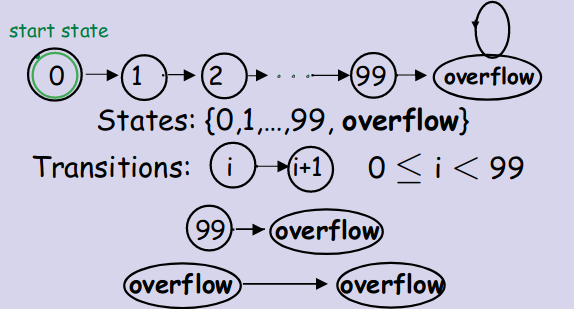
\includegraphics[width=1\textwidth]{../img/statemachine}
  \end{columns}
\end{frame}

\subsection{State Machines for Proofs}
\begin{frame}{State Machine for Proofs}{Robot 1.0}

  Imagine a robot moving forwards and backwards on a street. The robot has two speeds:
  \begin{itemize}
    \item The robot can move exactly {\bf five squares} forwards.
    \item The robot can move exactly {\bf three squares} backwards.
  \end{itemize}
  \bigskip

  If the robot starts from position 0, is it possible for it to reach position 4?
\end{frame}

\begin{frame}{State Machine for Proofs}{Robot 1.1}
  Imagine a robot moving forwards and backwards on a street. The robot has two speeds:
  \begin{itemize}
    \item The robot can move exactly {\bf nine squares} forwards.
    \item The robot can move exactly {\bf three squares} backwards.
  \end{itemize}
  \bigskip

  If the robot starts from position 0, is it possible for it to reach position 4?
\end{frame}

\begin{frame}{State Machine for Proofs}{Preserved Invariants}

  \structure{Preserved Invariants} are propositions that are always true, after {\bf any} transition of the state machine. We can use preserved invariants to prove which squares the robots can reach.

  \begin{block}{Robot 1.0}
    The position of robot 1.0 is always: $s_0 + 5a - 3b$
  \end{block}
  \begin{block}{Robot 1.1}
    The position of robot 1.1 is always: $s_0 + 9a - 3b$
    \begin{itemize}
      \item $s_0 + 9a - 3b = s_0 + 3(3a-b)$
      \item The position of robot 1.1 is always $s_0$ plus a multiple of 3; (\structure{Preserved Invariant})
      \item So it is impossible for robot 1.1 to reach 4 from 0.
    \end{itemize}
  \end{block}
\end{frame}


\begin{frame}{Induction with Preserved Invariants}

  Preserved Invariants can be used together with inductions to prove things about state machines:\bigskip

  \begin{itemize}
    \item Prove that $P(s)$ is a preserved invariant. This means that if $P(s)$ is true for some state $s$, then it will continue to be true after any transition.\medskip

    \item Prove that $P(s)$ is true for the initial state, $s_0$.\medskip

    \item Conclude that $P(s)$ is always true for the entire state machine.
  \end{itemize}\bigskip

  If $P(s)$ is a "correctness condition" of an algorithm, this method can be used to prove that an algorithm is correct.
\end{frame}


\begin{frame}{State Machine for Proofs}{Robot 2.0}

  Robot 2.0 can move on the diagonals of $\mathbb{Z}^2$: (+1,
  +1), (-1,-1), (+1,-1), (-1,+1). Starting from (0,0), is it possible for the robot to reach position (1,0)?

  \begin{center}
    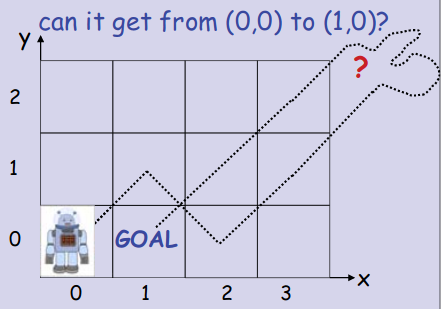
\includegraphics[width=0.4\textwidth]{../img/diag_robot}
  \end{center}

  \alert{QUIZ}: Try to prove this by yourself first!

\end{frame}


\begin{frame}{State Machine for Proofs}{Robot 2.0 -- Solution}

  We can show that a \structure{preserved invariant} of robot 2.0 is that the sum of its coordinates is always even (or always odd):\bigskip

  \begin{itemize}
  \item P(0,0) is true (0+0 is even).
  \item The steps of the robot are:
    \begin{itemize}
    \item $+1+1 = +2$: even + 2 is still even;
    \item $-1-1 = -2$: even - 2 is still even;
    \item $+1-1 = 0$: even + 0 is still even;
    \item $-1+1 = 0$: even + 0 is still even;
    \end{itemize}
  \end{itemize}
  \bigskip

  So we can see that the parity of the position is a \structure{preserved invariant}. Because the parities of (0,0) and (1,0) are different, it is impossible for robot 2.0 to go from (0,0) to (1,0).
\end{frame}

\begin{frame}{State Machines for Proofs}{Fast Exponentiation}

  This is the end for this lecture. I highly recommend that you watch lecture video 1.9.1 from MIT OCW for a final example with the Fast Exponentiation algorithm.\bigskip

  Summary of the third part: To prove that an algorithm is correct, we need to show that:
  \begin{itemize}
    \item Prove that if the algorihm is in a correct state, it will always stay in the correct state (preserved invariant);
    \item Prove that the algorithm can reach the correct state from the initial position;
    \item Prove that the algorithm stops at some point (not an infinite loop).
    \begin{itemize}
      \item We haven't talked about this part yet, but you can prove this by showing that some variable in the state machine is always decreasing.
    \end{itemize}
  \end{itemize}
\end{frame}


\begin{frame}{Slide Credits}
  These slides were made by Claus Aranha, 2020. You are welcome to copy, re-use and modify this material, following the CC-SA-NC license.
  \bigskip

  These slides are based on "Mathematics For Computer Science (Spring 2015)", by Albert Meyer and Adam Chlipala, MIT OpenCourseWare. \url{https://ocw.mit.edu}.
  \bigskip

  Individual images in some slides might have been made by other
  authors. Please see the following slides for information about these cases.
\end{frame}

\begin{frame}[allowframebreaks]{Image Credits}
  \printnotes
\end{frame}

\end{document}
